% Options for packages loaded elsewhere
% Options for packages loaded elsewhere
\PassOptionsToPackage{unicode}{hyperref}
\PassOptionsToPackage{hyphens}{url}
\PassOptionsToPackage{dvipsnames,svgnames,x11names}{xcolor}
%
\documentclass[
  twoside,
  symmetric]{tufte-book}
\usepackage{xcolor}
\usepackage{amsmath,amssymb}
\setcounter{secnumdepth}{-\maxdimen} % remove section numbering
\usepackage{iftex}
\ifPDFTeX
  \usepackage[T1]{fontenc}
  \usepackage[utf8]{inputenc}
  \usepackage{textcomp} % provide euro and other symbols
\else % if luatex or xetex
  \usepackage{unicode-math} % this also loads fontspec
  \defaultfontfeatures{Scale=MatchLowercase}
  \defaultfontfeatures[\rmfamily]{Ligatures=TeX,Scale=1}
\fi
\usepackage{lmodern}
\ifPDFTeX\else
  % xetex/luatex font selection
\fi
% Use upquote if available, for straight quotes in verbatim environments
\IfFileExists{upquote.sty}{\usepackage{upquote}}{}
\IfFileExists{microtype.sty}{% use microtype if available
  \usepackage[]{microtype}
  \UseMicrotypeSet[protrusion]{basicmath} % disable protrusion for tt fonts
}{}
\makeatletter
\@ifundefined{KOMAClassName}{% if non-KOMA class
  \IfFileExists{parskip.sty}{%
    \usepackage{parskip}
  }{% else
    \setlength{\parindent}{0pt}
    \setlength{\parskip}{6pt plus 2pt minus 1pt}}
}{% if KOMA class
  \KOMAoptions{parskip=half}}
\makeatother
% Make \paragraph and \subparagraph free-standing
\makeatletter
\ifx\paragraph\undefined\else
  \let\oldparagraph\paragraph
  \renewcommand{\paragraph}{
    \@ifstar
      \xxxParagraphStar
      \xxxParagraphNoStar
  }
  \newcommand{\xxxParagraphStar}[1]{\oldparagraph*{#1}\mbox{}}
  \newcommand{\xxxParagraphNoStar}[1]{\oldparagraph{#1}\mbox{}}
\fi
\ifx\subparagraph\undefined\else
  \let\oldsubparagraph\subparagraph
  \renewcommand{\subparagraph}{
    \@ifstar
      \xxxSubParagraphStar
      \xxxSubParagraphNoStar
  }
  \newcommand{\xxxSubParagraphStar}[1]{\oldsubparagraph*{#1}\mbox{}}
  \newcommand{\xxxSubParagraphNoStar}[1]{\oldsubparagraph{#1}\mbox{}}
\fi
\makeatother


\usepackage{longtable,booktabs,array}
\usepackage{calc} % for calculating minipage widths
% Correct order of tables after \paragraph or \subparagraph
\usepackage{etoolbox}
\makeatletter
\patchcmd\longtable{\par}{\if@noskipsec\mbox{}\fi\par}{}{}
\makeatother
% Allow footnotes in longtable head/foot
\IfFileExists{footnotehyper.sty}{\usepackage{footnotehyper}}{\usepackage{footnote}}
\makesavenoteenv{longtable}
\usepackage{graphicx}
\makeatletter
\newsavebox\pandoc@box
\newcommand*\pandocbounded[1]{% scales image to fit in text height/width
  \sbox\pandoc@box{#1}%
  \Gscale@div\@tempa{\textheight}{\dimexpr\ht\pandoc@box+\dp\pandoc@box\relax}%
  \Gscale@div\@tempb{\linewidth}{\wd\pandoc@box}%
  \ifdim\@tempb\p@<\@tempa\p@\let\@tempa\@tempb\fi% select the smaller of both
  \ifdim\@tempa\p@<\p@\scalebox{\@tempa}{\usebox\pandoc@box}%
  \else\usebox{\pandoc@box}%
  \fi%
}
% Set default figure placement to htbp
\def\fps@figure{htbp}
\makeatother





\setlength{\emergencystretch}{3em} % prevent overfull lines

\providecommand{\tightlist}{%
  \setlength{\itemsep}{0pt}\setlength{\parskip}{0pt}}



 
\usepackage[]{natbib}
\bibliographystyle{plainnat}


\usepackage{lipsum}
\usepackage{graphicx}
\graphicspath{{style-guide/graphics/}}
\newcommand{\TL}{Tufte-\LaTeX\xspace}
\newcommand{\newthought}[1]{\noindent\textsc{#1}}
\makeatletter
\@ifpackageloaded{caption}{}{\usepackage{caption}}
\AtBeginDocument{%
\ifdefined\contentsname
  \renewcommand*\contentsname{Table of contents}
\else
  \newcommand\contentsname{Table of contents}
\fi
\ifdefined\listfigurename
  \renewcommand*\listfigurename{List of Figures}
\else
  \newcommand\listfigurename{List of Figures}
\fi
\ifdefined\listtablename
  \renewcommand*\listtablename{List of Tables}
\else
  \newcommand\listtablename{List of Tables}
\fi
\ifdefined\figurename
  \renewcommand*\figurename{Figure}
\else
  \newcommand\figurename{Figure}
\fi
\ifdefined\tablename
  \renewcommand*\tablename{Table}
\else
  \newcommand\tablename{Table}
\fi
}
\@ifpackageloaded{float}{}{\usepackage{float}}
\floatstyle{ruled}
\@ifundefined{c@chapter}{\newfloat{codelisting}{h}{lop}}{\newfloat{codelisting}{h}{lop}[chapter]}
\floatname{codelisting}{Listing}
\newcommand*\listoflistings{\listof{codelisting}{List of Listings}}
\makeatother
\makeatletter
\makeatother
\makeatletter
\@ifpackageloaded{caption}{}{\usepackage{caption}}
\@ifpackageloaded{subcaption}{}{\usepackage{subcaption}}
\makeatother
\makeatletter
\@ifpackageloaded{sidenotes}{}{\usepackage{sidenotes}}
\@ifpackageloaded{marginnote}{}{\usepackage{marginnote}}
\makeatother
\usepackage{bookmark}
\IfFileExists{xurl.sty}{\usepackage{xurl}}{} % add URL line breaks if available
\urlstyle{same}
\hypersetup{
  pdftitle={A Tufte-Style Book},
  pdfauthor={The Tufte-LaTeX Developers},
  colorlinks=true,
  linkcolor={blue},
  filecolor={Maroon},
  citecolor={Blue},
  urlcolor={Blue},
  pdfcreator={LaTeX via pandoc}}


\title{A Tufte-Style Book}
\usepackage{etoolbox}
\makeatletter
\providecommand{\subtitle}[1]{% add subtitle to \maketitle
  \apptocmd{\@title}{\par {\large #1 \par}}{}{}
}
\makeatother
\subtitle{Thanks to Edward R. Tufte for his inspiration}
\author{The Tufte-LaTeX Developers}
\date{2025-05-24}
\begin{document}
% Front matter
\frontmatter

% Blank page
\blankpage

% Epigraphs page

% Title page
\maketitle

% Copyright page
\newpage
\begin{fullwidth}
~\vfill
\thispagestyle{empty}
\setlength{\parindent}{0pt}
\setlength{\parskip}{\baselineskip}
Copyright \copyright\ \the\year\ The Tufte-LaTeX Developers

\par\smallcaps{Published by Publisher of This Book}

\par\smallcaps{tufte-latex.github.io/tufte-latex/}

\par Licensed under the Apache License, Version 2.0 (the ``License''); you may not
use this file except in compliance with the License. You may obtain a copy
of the License at \url{http://www.apache.org/licenses/LICENSE-2.0}. Unless
required by applicable law or agreed to in writing, software distributed
under the License is distributed on an \smallcaps{``AS IS'' BASIS, WITHOUT
WARRANTIES OR CONDITIONS OF ANY KIND}, either express or implied. See the
License for the specific language governing permissions and limitations
under the License.

\par\textit{First printing, \monthyear}
\end{fullwidth}

% Table of contents


% Start main matter
\mainmatter

\mainmatter
\frontmatter

\openepigraph{The public is more familiar with bad design than good design. It is, in effect, conditioned to prefer bad design, because that is what it lives with. The new becomes threatening, the old reassuring.}{Paul Rand}

\vfill

\openepigraph{A designer knows that he has achieved perfection not when there is nothing left to add, but when there is nothing left to take away.}{Antoine de Saint-Exupéry}

\vfill

\openepigraph{...the designer of a new system must not only be the implementor and the first large-scale user; the designer should also write the first user manual... If I had not participated fully in all these activities, literally hundreds of improvements would never have been made, because I would never have thought of them or perceived why they were important.}{Donald E. Knuth}

\maketitle

\tableofcontents
\listoffigures  
\listoftables

\mainmatter

\chapter*{Introduction}\label{introduction}
\addcontentsline{toc}{chapter}{Introduction}

This sample book discusses the design of Edward Tufte's
books\citep{Tufte2001, Tufte1990, Tufte1997, Tufte2006} and the use of
the \texttt{tufte-book} and \texttt{tufte-handout} document classes.

\chapter{The Design of Tufte's Books}\label{ch:tufte-design}

\newthought{The pages} of a book are usually divided into three major
sections: the front matter (also called preliminary matter or prelim),
the main matter (the core text of the book), and the back matter (or end
matter).

\newthought{The front matter} of a book refers to all of the material
that comes before the main text.

\section{Sidenotes}\label{sidenotes}

One of the most prominent and distinctive features of this style is the
extensive use of sidenotes.\footnote{This is a sidenote that was entered
  using the footnote command.} There is a wide margin to provide ample
room for sidenotes and small figures.

\section{Figures and Tables}\label{figures-and-tables}

Images and graphics play an integral role in Tufte's work.

\begin{figure}[H]

{\centering \pandocbounded{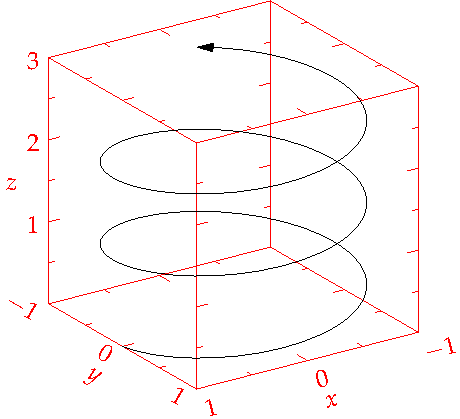
\includegraphics[keepaspectratio]{style-guide/graphics/helix.pdf}}

}

\caption{This is a margin figure. The helix is defined by
\(x = \cos(2\pi z)\), \(y = \sin(2\pi z)\), and \(z = [0, 2.7]\).}

\end{figure}%

Full page-width figures may be placed using the \texttt{.column-page}
class.

\begin{figure*}

\begin{figure}[H]

{\centering \pandocbounded{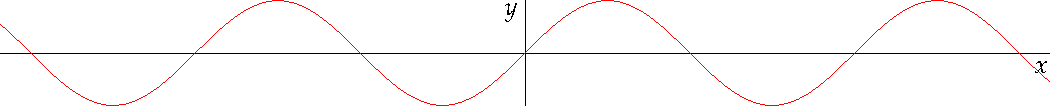
\includegraphics[keepaspectratio]{style-guide/graphics/sine.pdf}}

}

\caption{This graph shows \(y = \sin x\) from about \(x = [-10, 10]\).
\emph{Notice that this figure takes up the full page width.}}

\end{figure}%

\end{figure*}%

\chapter*{References}\label{references}
\addcontentsline{toc}{chapter}{References}

\renewcommand{\bibsection}{}
\bibliography{style-guide/sample-handout.bib}


\backmatter


% Back matter
\backmatter




\end{document}
